% Generated by scripts/build-paper-tracked.sh; do not edit.
%DIF 1c1
%DIF LATEXDIFF DIFFERENCE FILE
%DIF DEL /Users/yehezkielgunawan/Documents/Personal Project/jev-paper/paper/.build/tracked/original.tex   Thu Nov  5 20:28:11 2026
%DIF ADD /Users/yehezkielgunawan/Documents/Personal Project/jev-paper/paper/.build/tracked/revised.tex    Thu Nov  5 20:28:11 2026
%DIF < % Blinded review manuscript. Compile from paper/ with latexmk -pdf manuscript.tex.
%DIF -------
% Author-identified manuscript. Compile from paper/ with latexmk -pdf manuscript.tex. %DIF > 
%DIF -------
% Numerical results: ../results/metrics/; data audit: ../results/audit/.
\documentclass{llncs}
\usepackage{graphicx}
\usepackage{xurl} %DIF > 
%DIF PREAMBLE EXTENSION ADDED BY LATEXDIFF
%DIF UNDERLINE PREAMBLE %DIF PREAMBLE
\RequirePackage[normalem]{ulem} %DIF PREAMBLE
\RequirePackage{color}\definecolor{RED}{rgb}{1,0,0}\definecolor{BLUE}{rgb}{0,0,1} %DIF PREAMBLE
\providecommand{\DIFadd}[1]{{\protect\color{blue}\uwave{#1}}} %DIF PREAMBLE
\providecommand{\DIFdel}[1]{{\protect\color{red}\sout{#1}}} %DIF PREAMBLE
%DIF SAFE PREAMBLE %DIF PREAMBLE
\providecommand{\DIFaddbegin}{} %DIF PREAMBLE
\providecommand{\DIFaddend}{} %DIF PREAMBLE
\providecommand{\DIFdelbegin}{} %DIF PREAMBLE
\providecommand{\DIFdelend}{} %DIF PREAMBLE
\providecommand{\DIFmodbegin}{} %DIF PREAMBLE
\providecommand{\DIFmodend}{} %DIF PREAMBLE
%DIF FLOATSAFE PREAMBLE %DIF PREAMBLE
\providecommand{\DIFaddFL}[1]{\DIFadd{#1}} %DIF PREAMBLE
\providecommand{\DIFdelFL}[1]{\DIFdel{#1}} %DIF PREAMBLE
\providecommand{\DIFaddbeginFL}{} %DIF PREAMBLE
\providecommand{\DIFaddendFL}{} %DIF PREAMBLE
\providecommand{\DIFdelbeginFL}{} %DIF PREAMBLE
\providecommand{\DIFdelendFL}{} %DIF PREAMBLE
\providecommand{\DIFscaledelfig}{0.5}
%DIF HIGHLIGHTGRAPHICS PREAMBLE %DIF PREAMBLE
\RequirePackage{settobox} %DIF PREAMBLE
\RequirePackage{letltxmacro} %DIF PREAMBLE
\newsavebox{\DIFdelgraphicsbox} %DIF PREAMBLE
\newlength{\DIFdelgraphicswidth} %DIF PREAMBLE
\newlength{\DIFdelgraphicsheight} %DIF PREAMBLE
% store original definition of \includegraphics %DIF PREAMBLE
\LetLtxMacro{\DIFOincludegraphics}{\includegraphics} %DIF PREAMBLE
\providecommand{\DIFaddincludegraphics}[2][]{{\color{blue}\fbox{\DIFOincludegraphics[#1]{#2}}}} %DIF PREAMBLE
\providecommand{\DIFdelincludegraphics}[2][]{% %DIF PREAMBLE
\sbox{\DIFdelgraphicsbox}{\DIFOincludegraphics[#1]{#2}}% %DIF PREAMBLE
\settoboxwidth{\DIFdelgraphicswidth}{\DIFdelgraphicsbox} %DIF PREAMBLE
\settoboxtotalheight{\DIFdelgraphicsheight}{\DIFdelgraphicsbox} %DIF PREAMBLE
\scalebox{\DIFscaledelfig}{% %DIF PREAMBLE
\parbox[b]{\DIFdelgraphicswidth}{\usebox{\DIFdelgraphicsbox}\\[-\baselineskip] \rule{\DIFdelgraphicswidth}{0em}}\llap{\resizebox{\DIFdelgraphicswidth}{\DIFdelgraphicsheight}{% %DIF PREAMBLE
\setlength{\unitlength}{\DIFdelgraphicswidth}% %DIF PREAMBLE
\begin{picture}(1,1)% %DIF PREAMBLE
\thicklines\linethickness{2pt} %DIF PREAMBLE
{\color[rgb]{1,0,0}\put(0,0){\framebox(1,1){}}}% %DIF PREAMBLE
{\color[rgb]{1,0,0}\put(0,0){\line( 1,1){1}}}% %DIF PREAMBLE
{\color[rgb]{1,0,0}\put(0,1){\line(1,-1){1}}}% %DIF PREAMBLE
\end{picture}% %DIF PREAMBLE
}\hspace*{3pt}}} %DIF PREAMBLE
} %DIF PREAMBLE
\LetLtxMacro{\DIFOaddbegin}{\DIFaddbegin} %DIF PREAMBLE
\LetLtxMacro{\DIFOaddend}{\DIFaddend} %DIF PREAMBLE
\LetLtxMacro{\DIFOdelbegin}{\DIFdelbegin} %DIF PREAMBLE
\LetLtxMacro{\DIFOdelend}{\DIFdelend} %DIF PREAMBLE
\DeclareRobustCommand{\DIFaddbegin}{\DIFOaddbegin \let\includegraphics\DIFaddincludegraphics} %DIF PREAMBLE
\DeclareRobustCommand{\DIFaddend}{\DIFOaddend \let\includegraphics\DIFOincludegraphics} %DIF PREAMBLE
\DeclareRobustCommand{\DIFdelbegin}{\DIFOdelbegin \let\includegraphics\DIFdelincludegraphics} %DIF PREAMBLE
\DeclareRobustCommand{\DIFdelend}{\DIFOaddend \let\includegraphics\DIFOincludegraphics} %DIF PREAMBLE
\LetLtxMacro{\DIFOaddbeginFL}{\DIFaddbeginFL} %DIF PREAMBLE
\LetLtxMacro{\DIFOaddendFL}{\DIFaddendFL} %DIF PREAMBLE
\LetLtxMacro{\DIFOdelbeginFL}{\DIFdelbeginFL} %DIF PREAMBLE
\LetLtxMacro{\DIFOdelendFL}{\DIFdelendFL} %DIF PREAMBLE
\DeclareRobustCommand{\DIFaddbeginFL}{\DIFOaddbeginFL \let\includegraphics\DIFaddincludegraphics} %DIF PREAMBLE
\DeclareRobustCommand{\DIFaddendFL}{\DIFOaddendFL \let\includegraphics\DIFOincludegraphics} %DIF PREAMBLE
\DeclareRobustCommand{\DIFdelbeginFL}{\DIFOdelbeginFL \let\includegraphics\DIFdelincludegraphics} %DIF PREAMBLE
\DeclareRobustCommand{\DIFdelendFL}{\DIFOaddendFL \let\includegraphics\DIFOincludegraphics} %DIF PREAMBLE
%DIF COLORLISTINGS PREAMBLE %DIF PREAMBLE
\RequirePackage{listings} %DIF PREAMBLE
\RequirePackage{color} %DIF PREAMBLE
\lstdefinelanguage{DIFcode}{ %DIF PREAMBLE
%DIF DIFCODE_UNDERLINE %DIF PREAMBLE
  moredelim=[il][\color{red}\sout]{\%DIF\ <\ }, %DIF PREAMBLE
  moredelim=[il][\color{blue}\uwave]{\%DIF\ >\ } %DIF PREAMBLE
} %DIF PREAMBLE
\lstdefinestyle{DIFverbatimstyle}{ %DIF PREAMBLE
	language=DIFcode, %DIF PREAMBLE
	basicstyle=\ttfamily, %DIF PREAMBLE
	columns=fullflexible, %DIF PREAMBLE
	keepspaces=true %DIF PREAMBLE
} %DIF PREAMBLE
\lstnewenvironment{DIFverbatim}[1][]{\lstset{style=DIFverbatimstyle}}{} %DIF PREAMBLE
\lstnewenvironment{DIFverbatim*}[1][]{\lstset{style=DIFverbatimstyle,showspaces=true}}{} %DIF PREAMBLE
\lstset{extendedchars=\true,inputencoding=utf8}

%DIF END PREAMBLE EXTENSION ADDED BY LATEXDIFF

\begin{document}
\sloppy


\title{Leakage-Aware Transaction Risk Classification with Jev and Tree Ensembles}
\titlerunning{Leakage-Aware Transaction Risk Classification}
\author{\DIFaddbegin \DIFadd{Yehezkiel Gunawan }\and \DIFadd{Tanty Oktavia}\DIFaddend }
\DIFaddbegin \authorrunning{Y. Gunawan and T. Oktavia}
\DIFaddend \institute{\DIFaddbegin \DIFadd{Information Systems Management Department}\\
\DIFadd{Binus Graduate Programs -- Master of Information Systems Management}\\
\DIFadd{Bina Nusantara University}\\
\DIFadd{Jl. K. H. Syahdan No. 9, Kemanggisan, Palmerah, Jakarta 11480, Indonesia}\DIFaddend }
\maketitle
\begin{center}\small Revision markup: \DIFadd{blue underlined text is added}; \DIFdel{red struck-through text is deleted}. Changed figures are shown with graphical markup.\end{center}


\begin{abstract}
\DIFdelbegin \DIFdel{Pretrained decision services can return a risk decision without fitting on the target dataset, but their usefulness depends on whether the supplied transaction attributes contain information about the outcome}\DIFdelend \DIFaddbegin \DIFadd{Risk screening for accounting transactions requires information available before an incident is recorded}\DIFaddend . We compare \DIFdelbegin \DIFdel{a hosted}\DIFdelend \DIFaddbegin \DIFadd{the hosted, pretrained }\DIFaddend Jev decision service with tuned Random Forest and XGBoost classifiers on a simulated accounting-transaction dataset. All systems receive the same 12 leakage-screened features for 2,000 held-out records; the \DIFdelbegin \DIFdel{tree models }\DIFdelend \DIFaddbegin \DIFadd{trees }\DIFaddend are trained on 8,000 labeled records, whereas Jev receives no dataset-specific training examples. Three post-event columns that perfectly identify the outcome are excluded. On the held-out set (14.5\% positive), ROC-AUC is 0.503 for Random Forest, 0.515 for XGBoost, and 0.492 for Jev. Jev attains 0.700 recall but only 0.141 precision; its Brier score is 0.459, compared with 0.243 and 0.244 for the \DIFdelbegin \DIFdel{tree models. Restricting Jev predictions by its reported confidence reduces automatic-decision coverage without improving accuracyamong accepted cases at the evaluated thresholds. These results do not establish that one model family is universally preferable. They show that a leakage-aware evaluation of this single simulated dataset yields weak discrimination for all three systems, and that confidence-based deferral cannot be assumed to rescue an uninformative decision signal}\DIFdelend \DIFaddbegin \DIFadd{trees. Exploratory probability-threshold analysis exposes alert-volume trade-offs rather than improved ranking. Jev confidence ranks correct above incorrect decisions with AUC 0.434 (95\% bootstrap interval }[\DIFadd{0.407, 0.461}]\DIFadd{); its six evaluated deferral cutoffs reduce coverage without increasing accepted-case accuracy}\DIFaddend . \DIFaddbegin \DIFadd{Confidence selection favors positive predictions despite low incident prevalence. These findings characterize one simulated dataset and one service version, not a universal model-family ranking or a causal account of the models' errors.
}\DIFaddend 

\keywords{Tabular classification \and Financial risk \and Data leakage \and Probability reliability \and Selective prediction}
\end{abstract}

\section{Introduction}

Transaction risk screening is a structured decision problem: an automated system must make a decision using information available when a transaction is assessed, not fields recorded only after an incident is classified. The distinction matters in a dataset that mixes transaction attributes with incident descriptions. An evaluation that includes the latter can report impressive scores while answering an easier, operationally invalid question. Recent financial-risk benchmarks likewise emphasize the evaluation protocol and leakage control rather than model scores in isolation~\cite{mishra2026erp,zeng2026fraudbench}.

\DIFdelbegin \DIFdel{Random Forest and XGBoost are established supervised choices for tabular classification~\mbox{%DIFAUXCMD
\cite{breiman2001forests,chen2016xgboost}}\hskip0pt%DIFAUXCMD
. Large tabular benchmarks support strong tree baselines but also show that results vary with datasets and tuning~\mbox{%DIFAUXCMD
\cite{grinsztajn2022trees,mcelfresh2023tabzilla}}\hskip0pt%DIFAUXCMD
. Pretrained models offer another decision mechanism. A tabular foundation model such as TabPFN can exploit labeled in-context examples~\mbox{%DIFAUXCMD
\cite{hollmann2025tabpfn}}\hskip0pt%DIFAUXCMD
; zero-shot language-model studies investigate predictions without those examples and report mixed behavior~\mbox{%DIFAUXCMD
\cite{grushina2026llmtab,garnelo2026tabular}}\hskip0pt%DIFAUXCMD
. The hosted Jev system used here returns a structured binary choice and scores from a single transaction state. We do not assume that Jev has the architecture , training procedure, or in-context setting of any of these published systems}\DIFdelend \DIFaddbegin \DIFadd{Hosted services can make decisions without fitting on the target dataset, whereas supervised classifiers learn from its labeled records. Matching inputs is therefore necessary but does not match supervision. We compare Jev with Random Forest and XGBoost to examine these decision settings, not to isolate architecture effects}\DIFaddend .

Classification accuracy alone is especially difficult to interpret with a minority risk class: rejecting every case as non-risk can produce high accuracy while missing every incident. Precision--recall analysis addresses this imbalance~\cite{davis2006pr}. A second issue is probability reliability: a ranking metric does not establish that predicted probabilities match event frequencies~\cite{guo2017calibration,haotian2023recal}. A third is whether a separate confidence estimate identifies cases suitable for automatic decisions rather than human review~\cite{singh2026abstention}.

This study asks four questions on one common held-out test set: (RQ1) how do the systems classify risk incidents; (RQ2) how reliable are their positive-class probabilities; (RQ3) does Jev confidence-based deferral improve accepted-case performance; and (RQ4) what latency trade-off accompanies local and hosted inference? The contribution is \DIFdelbegin \DIFdel{an empirical , leakage-aware comparison across these dimensions, including }\DIFdelend \DIFaddbegin \DIFadd{a reproducible empirical audit combining leakage screening, supervised and task-untrained decision settings, }\DIFaddend a prevalence-only reference\DIFdelbegin \DIFdel{classifier. We report the negative result when observable inputs do not support useful discrimination}\DIFdelend \DIFaddbegin \DIFadd{, paired uncertainty estimates, and confidence-error diagnostics. It is not a new classifier or abstention algorithm. The original decisions and prompt remain fixed; additional operating-point analyses are explicitly exploratory.
}

\section{\DIFadd{Related Work and Research Gap}}\label{sec:related}

\textbf{\DIFadd{Fraud and transaction-risk detection.}} \DIFadd{Realistic credit-card fraud modeling has been studied as an operational learning problem~\mbox{%DIFAUXCMD
\cite{dalpozzolo2018fraud}}\hskip0pt%DIFAUXCMD
. Recent work evaluates validation-selected model fusion on IEEE-CIS~\mbox{%DIFAUXCMD
\cite{han2026fusion} }\hskip0pt%DIFAUXCMD
and optimized explainable boosting on credit-card data~\mbox{%DIFAUXCMD
\cite{fazel2026ebm}}\hskip0pt%DIFAUXCMD
. These studies concern fraud labels and supervised detection, whereas our target includes simulated accounting risk incidents more broadly. Their reported scores cannot serve as numerical baselines on different records, labels, or splits. Random Forest and XGBoost are established tabular methods~\mbox{%DIFAUXCMD
\cite{breiman2001forests,chen2016xgboost}}\hskip0pt%DIFAUXCMD
; broad benchmarks further show that dataset properties and hyperparameter tuning can matter as much as model-family choice~\mbox{%DIFAUXCMD
\cite{grinsztajn2022trees,mcelfresh2023tabzilla}}\hskip0pt%DIFAUXCMD
.
}

\textbf{\DIFadd{Leakage-aware evaluation.}} \DIFadd{Kaufman et al.~\mbox{%DIFAUXCMD
\cite{kaufman2012leakage} }\hskip0pt%DIFAUXCMD
define leakage in terms of information unavailable for legitimate prediction, rather than merely suspicious correlations. ERP-RiskBench applies time- and group-aware evaluation to financial risk~\mbox{%DIFAUXCMD
\cite{mishra2026erp}}\hskip0pt%DIFAUXCMD
. FraudBench shows that financial adversarial-robustness conclusions depend on feasibility and deployment constraints~\mbox{%DIFAUXCMD
\cite{zeng2026fraudbench}}\hskip0pt%DIFAUXCMD
; its focus is not ordinary target leakage. Together, these studies motivate explicit operational assumptions. Our narrower audit removes direct target encodings and isolates a common split; it does not establish the temporal or institutional validity of the remaining attributes.
}

\textbf{\DIFadd{Pretrained decision models.}} \DIFadd{TabPFN uses labeled in-context examples and pretraining over synthetic prediction tasks~\mbox{%DIFAUXCMD
\cite{hollmann2025tabpfn}}\hskip0pt%DIFAUXCMD
. TabLens investigates conditions under which zero- and few-shot language models can substitute for labeled examples~\mbox{%DIFAUXCMD
\cite{grushina2026llmtab}}\hskip0pt%DIFAUXCMD
. Garnelo and Czarnecki examine dimensionality-related failures in a different regime that supplies training and test data in context~\mbox{%DIFAUXCMD
\cite{garnelo2026tabular}}\hskip0pt%DIFAUXCMD
. Neither regime is interchangeable with Jev's single-row}\DIFaddend , \DIFdelbegin \DIFdel{rather than selecting an outcome threshold or prompt after inspecting the test labels. }\DIFdelend \DIFaddbegin \DIFadd{no-example setting. Provatas and Georgakopoulos-Soares audit Jev itself on biology and biosecurity-relevant multiple-choice tasks~\mbox{%DIFAUXCMD
\cite{provatas2026systemone}}\hskip0pt%DIFAUXCMD
; they find task-dependent reliability and explain why its confidence field is not a raw probability of correctness. Their results motivate, but do not answer, a transaction-risk evaluation.
}\DIFaddend 

\DIFaddbegin \textbf{\DIFadd{Reliability and selective prediction.}} \DIFadd{Probability calibration~\mbox{%DIFAUXCMD
\cite{guo2017calibration,haotian2023recal} }\hskip0pt%DIFAUXCMD
differs from discrimination. Calibration scores also require context about predictive performance~\mbox{%DIFAUXCMD
\cite{chidambaram2025reassessing}}\hskip0pt%DIFAUXCMD
. Selective classification trades coverage against accepted-case risk~\mbox{%DIFAUXCMD
\cite{geifman2017selective}}\hskip0pt%DIFAUXCMD
; cost-sensitive abstention additionally accounts for minority classes and review budgets~\mbox{%DIFAUXCMD
\cite{singh2026abstention}}\hskip0pt%DIFAUXCMD
. We use these established evaluation ideas, without claiming risk guarantees or measuring a human-review system.
}

\textbf{\DIFadd{Research gap.}} \DIFadd{The cited work does not establish whether Jev's single-row decisions and confidence support incident screening on this simulated accounting dataset after direct target encodings are removed, relative to tuned supervised trees receiving the same permitted attributes. Our contribution addresses that bounded empirical question and diagnoses the negative result through probability thresholds, confidence--correctness ranking, subset composition, and matched-coverage random-selection references. It does not claim novelty for leakage control or confidence-based deferral themselves. The 2026 arXiv studies above are preprints, not independent validation of our findings.
}

\DIFaddend \section{Method\DIFaddbegin \DIFadd{ology}\DIFaddend  }\DIFaddbegin \label{sec:method}
\DIFaddend 

\subsection{Dataset and Feature Availability}

We use version 1 of the Financial Transaction and Risk Management Dataset published by Ziya on Kaggle under CC0~\cite{ziya2025dataset}. Its description says it was designed to \emph{simulate} accounting transactions and risk events\DIFdelbegin \DIFdel{. Accordingly, the dataset is a simulation, not evidence of performance in a financial institution. }\DIFdelend \DIFaddbegin \DIFadd{, including fraud, errors, and misstatements; it is not a collection of independently verified institutional incidents. We did not generate the data. }\DIFaddend The supplied CSV contains 10,000 rows and 18 columns, including a binary \texttt{Risk\_Incident} label (1,448 positives; 14.48\%). The audit finds no duplicate records, duplicate transaction IDs, or empty CSV values. Transaction dates range from January 2024 to January 2025. The \DIFdelbegin \DIFdel{source dataset description does not specify an independently validated incident-label generation rule.
}\DIFdelend \DIFaddbegin \DIFadd{publisher's description provides neither a generation script, sampling distributions, nor a rule linking pre-event attributes to incident labels. We therefore document the observed file rather than invent a generation mechanism or assume that the permitted features determine the target.
}\DIFaddend 

The audit shows that \texttt{Risk\_Type}, \texttt{Incident\_Severity}, and \texttt{Error\_Code} each perfectly separate the binary classes in this file: their non-incident placeholder and incident values encode the target. None enters a classifier or Jev state. We also exclude transaction/account/user identifiers and \texttt{Counterparty} to avoid memorizing high-cardinality identities; \texttt{Currency} is constant. The original \texttt{Date} becomes year, month, day of week, and day of year. The remaining 12 features comprise transaction type, category, payment method, IP region, amount, system latency, login frequency, failed attempts, and these four calendar components. Jev and the supervised baselines use the same feature names and underlying values, although their representations differ. Availability of system latency and behavioral fields at the instant of screening is assumed, not independently established by the dataset publisher. The parser preserves the valid literal \texttt{NA} IP-region code and does not misinterpret the \texttt{None} placeholder in excluded columns as missing data.

\DIFaddbegin \DIFadd{The 12 inputs are the retained transaction descriptors, not a top-12 selection based on test performance. Transaction type, category, payment method, and amount describe the transaction; IP region and login/failed-attempt counts provide candidate access-context signals; latency describes processing context. Calendar components preserve date information in a common numeric representation. These are plausible screening inputs, not validated causal risk factors. Exclusions follow target encoding, identity memorization concerns, or constancy, rather than a feature-importance search. Calendar redundancy and the assumed availability of processing metadata remain limitations.
}

\DIFaddend \begin{table}[t]
\caption{Dataset and leakage-aware evaluation protocol. Test counts come from the frozen prediction files.}\label{tab:data}
\centering\small
\resizebox{\textwidth}{!}{\begin{tabular}{ll}
\hline
Dataset / target & Simulated accounting transactions / \texttt{Risk\_Incident} \\
Rows / positive labels & 10,000 / 1,448 (14.48\%) \\
Training / test rows & 8,000 / 2,000 (seed 42, stratified) \\
Positive / negative test labels & 290 / 1,710 \\
Model inputs & 4 categorical + 8 numeric/derived fields \\
Target-encoding fields excluded & \texttt{Risk\_Type}, \texttt{Incident\_Severity}, \texttt{Error\_Code} \\
\hline
\end{tabular}}
\end{table}

\subsection{Split and Model Configurations}

A single stratified 80/20 split with random seed 42 fixes the held-out test IDs for every method. Supervised preprocessing is fitted inside each training pipeline: median imputation for numeric fields, most-frequent imputation and one-hot encoding for categorical fields, with unseen categories ignored. On the training portion only, five-fold shuffled stratified cross-validation selects hyperparameters by average precision. Random Forest uses balanced class weights; its selected configuration has 200 trees, maximum depth 10, and minimum split size 5. XGBoost uses \texttt{scale\_pos\_weight} equal to the training negative/positive ratio, 0.8 row and column subsampling, histogram tree construction, and a selected 200 trees, depth 3, and learning rate 0.03. Its evaluation metric during fitting is log loss. The chosen parameter values, package versions, and split are recorded in the experiment metadata. A \texttt{DummyClassifier} predicting according to training prevalence supplies a non-discriminating reference. Supervised hard predictions use a fixed positive-probability threshold strictly greater than 0.5; this threshold was not tuned on the test set.

\DIFdelbegin \DIFdel{Jev is }\DIFdelend \DIFaddbegin \DIFadd{The complete Random Forest grid is tree count $\{200,500\}$, maximum depth $\{\mathrm{unlimited},10,20\}$, and minimum split size $\{2,5\}$ (12 combinations). The XGBoost grid is tree count $\{200,500\}$, maximum depth $\{3,6\}$, and learning rate $\{0.03,0.1\}$ (8 combinations). Cross-validation uses seed 42 and refits each best pipeline on all 8,000 training rows, with preprocessing learned within each fold during selection. Best mean cross-validation AP is 0.1562 for Random Forest and 0.1513 for XGBoost. These bounded searches are not exhaustive optimization. Recorded training versions are scikit-learn 1.9.1, XGBoost 3.4.1, and pandas 3.0.6.
}

\subsection{\DIFadd{Jev Hosted Decision Service}}\label{sec:jev}

\DIFadd{Jev is TypeSafe's pretrained decision model, accessed here through the hosted System One API and Python SDK, rather than a classifier fitted by the authors. The interface evaluates application state against typed questions and returns structured decisions~\mbox{%DIFAUXCMD
\cite{typesafe2026choice}}\hskip0pt%DIFAUXCMD
. The vendor describes non-generative inference; we do not independently inspect its architecture, training corpus, or internal computation. Our reproducible specification is therefore the observable interface, input state, question, and returned model version, not an implementation-level account of its internals.
}

\DIFadd{Jev is }\DIFaddend evaluated as a hosted, task-untrained decision service. For each held-out row, the same 12 feature values are serialized as a named state and submitted with a binary \texttt{Choice} question: ``Classify the transaction in the supplied state. Choose risk\_incident when the available transaction information indicates that this transaction should be flagged as a risk incident; otherwise choose no\_risk\_incident. Use only the supplied state.'' The two choice criteria restate whether the transaction should or should not be flagged. No training labels, exemplars, or excluded incident fields are supplied. The client requested \texttt{jev-latest}; the pilot and saved responses identify the returned model as \texttt{jev-1.13.0} (pilot recorded 25 September 2026). The question version is \texttt{binary-risk-choice-v1}. The chosen option determines Jev's hard prediction. Its \texttt{probabilities["risk\_incident"]} supplies the positive-class probability, while the separately returned \texttt{confidence} field is used only for the deferral analysis. We do not equate that field with the positive-class probability or assert that it is a calibrated probability of correctness. Unlike Random Forest and XGBoost, Jev did not fit on this dataset's training labels; consequently this is a comparison of decision settings, not a controlled comparison of learning algorithms.

\DIFaddbegin \DIFadd{The SDK's }\texttt{\DIFadd{system\_one}} \DIFadd{method calls }\url{https://api.typesafe.ai/v1/systemone} \DIFadd{with state and a question map. Current vendor documentation defines Choice confidence as $(p_{\max}-1/n)/(1-1/n)$ for $n$ options~\mbox{%DIFAUXCMD
\cite{typesafe2026confidence}}\hskip0pt%DIFAUXCMD
; for two normalized options this is $|2p-1|$, not the probability that the decision is correct. We audit this relationship against saved outputs rather than assuming that current documentation establishes historical implementation details. Responses are cached by sample ID and input-state fingerprint; full inference verifies the dataset fingerprint and resolved version. Reanalysis uses saved predictions and makes no new service calls.
}

\DIFaddend \subsection{Measurements and Uncertainty}

We report accuracy, positive-class precision, recall, F1, ROC-AUC, average precision (AP), and Brier score. AP summarizes the precision--recall ranking; its non-informative reference level is approximately the positive prevalence. For labels $y_i\in\{0,1\}$ and predicted positive probabilities $p_i$, the Brier score is $N^{-1}\sum_i(p_i-y_i)^2$ (lower is better). We also inspect ten-quantile-bin reliability plots. Brier score is a proper scoring rule that mixes calibration and refinement; a low score \emph{alone} does not prove useful discrimination or good calibration~\cite{chidambaram2025reassessing}.

For Jev, we retain a prediction when its reported confidence is at least $t\in\{0.50,0.60,0.70,0.80,0.90,0.95\}$. Coverage is the retained fraction of all 2,000 test records; performance is computed \emph{only among retained records}, and the others count as prospective human-review cases. These thresholds describe test-set behavior rather than an independently validated deployment policy. For uncertainty, 1,000 seeded bootstrap resamples of shared held-out IDs provide percentile 95\% intervals for individual metrics and paired model differences; they do not measure variation from a new train/test split or new Jev request. Local model latency is wall-clock time for one row's pipeline \texttt{predict\_proba}; Jev latency is the hosted API round trip, including network effects. Both are summarized by mean, median, and 95th percentile, but are not measurements of identical compute boundaries.

\DIFaddbegin \DIFadd{The revision adds nine exploratory probability thresholds for every model: $u=0.1,0.2,\ldots,0.9$, using $\hat y=\mathbf{1}[p>u]$. Unlike confidence cutoffs, these change the predicted label rather than decide which existing predictions to retain. Jev's returned choice remains its primary decision. We report all nine operating points without selecting a best test-set threshold; undefined precision/recall/F1 denominators are assigned zero, while ranking metrics on single-class subsets are undefined.
}

\DIFadd{To investigate deferral, we compute ROC-AUC with correctness as the binary target and confidence as the ranking score (0.5 means chance error discrimination). We report accepted-subset prevalence, predicted-positive fraction, and selective risk, defined as accepted-case error rate. The full risk--coverage curve retains complete groups of tied confidence scores. At the six fixed cutoffs, shared-row bootstrap draws recompute acceptance and provide pointwise intervals for conditional metrics and paired accepted-minus-unfiltered accuracy. Empty accepted draws are omitted for undefined conditional metrics and their valid resample counts are exported. A separate seeded random-selection reference draws uniform subsets without replacement at each observed accepted count, using 1,000 hypergeometric draws of correct-decision counts; its central 95\% range is a conditional randomization reference, }\emph{\DIFadd{not}} \DIFadd{a confidence interval. Expected random-selection accuracy equals unfiltered accuracy. Confidence bins use five equal-width intervals, with the last including 1. These exploratory intervals are not simultaneous or multiplicity-adjusted guarantees.
}

\subsection{\DIFadd{Reanalysis Artifacts}}\label{sec:artifacts}

\DIFadd{The project repository, containing the experimental code and reproducibility instructions, is available at }\url{https://github.com/yehezkielgunawan/jev-paper}\DIFadd{.
}

\DIFadd{Code is in }\path{src/jev_risk/}\DIFadd{. Running }\texttt{\DIFadd{uv run jev-risk}} \texttt{\DIFadd{evaluate}} \DIFadd{reads frozen prediction CSVs and exports tables and figures to }\path{results/}\DIFadd{. Experiment metadata records split IDs, dataset SHA-256, tuning settings, and returned service version. The offline manifest adds prediction-file hashes, analysis version, thresholds, seeds, bootstrap count, and analysis package versions. Reanalysis needs no API credentials; recreating Jev outputs requires service access and availability of the historical model. The source dataset is public, but exact offline reproduction also requires the saved predictions and analysis code.
}

\DIFaddend \section{Results}

\subsection{Classification and Probability Scores}

Table~\ref{tab:main} reports the full 2,000-row held-out evaluation. All three non-dummy ROC-AUC values are close to 0.5 and their 95\% bootstrap intervals include 0.5: Random Forest 0.503 [0.466, 0.541], XGBoost 0.515 [0.479, 0.555], and Jev 0.492 [0.456, 0.533]. AP ranges from 0.151 to 0.164, near the 0.145 test prevalence. The paired XGBoost-minus-Jev ROC-AUC interval is [-0.027, 0.071]; the paired F1 interval is [-0.046, 0.012]. Neither supports a clear difference on these two metrics at this sample size. This is not evidence of equivalence.

\begin{table}[t]
\caption{Held-out classification results ($N=2{,}000$). AP is average precision, not trapezoidal PR area; BS is Brier score (lower is better). The dummy predicts no incident for all rows.}\label{tab:main}
\centering\scriptsize
\resizebox{\textwidth}{!}{\begin{tabular}{lrrrrrrr}
\hline
Model & Accuracy & Precision & Recall & F1 & ROC-AUC & AP & BS$\downarrow$ \\
\hline
Prevalence dummy & .855 & .000 & .000 & .000 & .500 & .145 & .124 \\
Random Forest & .626 & .152 & .345 & .211 & .503 & .152 & .243 \\
XGBoost & .542 & .145 & .441 & .218 & .515 & .164 & .244 \\
Jev & .339 & .141 & .700 & .235 & .492 & .151 & .459 \\
\hline
\end{tabular}}
\end{table}

The dummy's 0.855 accuracy results from predicting the majority class and missing all 290 incidents. Jev predicts risk for 1,438 of 2,000 transactions (71.9\%): 203 true positives, 1,235 false positives, 87 false negatives, and 475 true negatives. Random Forest yields 100 true positives and 559 false positives; XGBoost yields 128 and 754, respectively. Jev's higher recall and F1 at the fixed operating point therefore coincide with many extra alerts, while its ROC ranking remains near chance. The precision--recall curves in Fig.~\ref{fig:pr} show how precision varies with recall.

\begin{figure}[t]
\centering
\DIFdelbeginFL \DIFdelFL{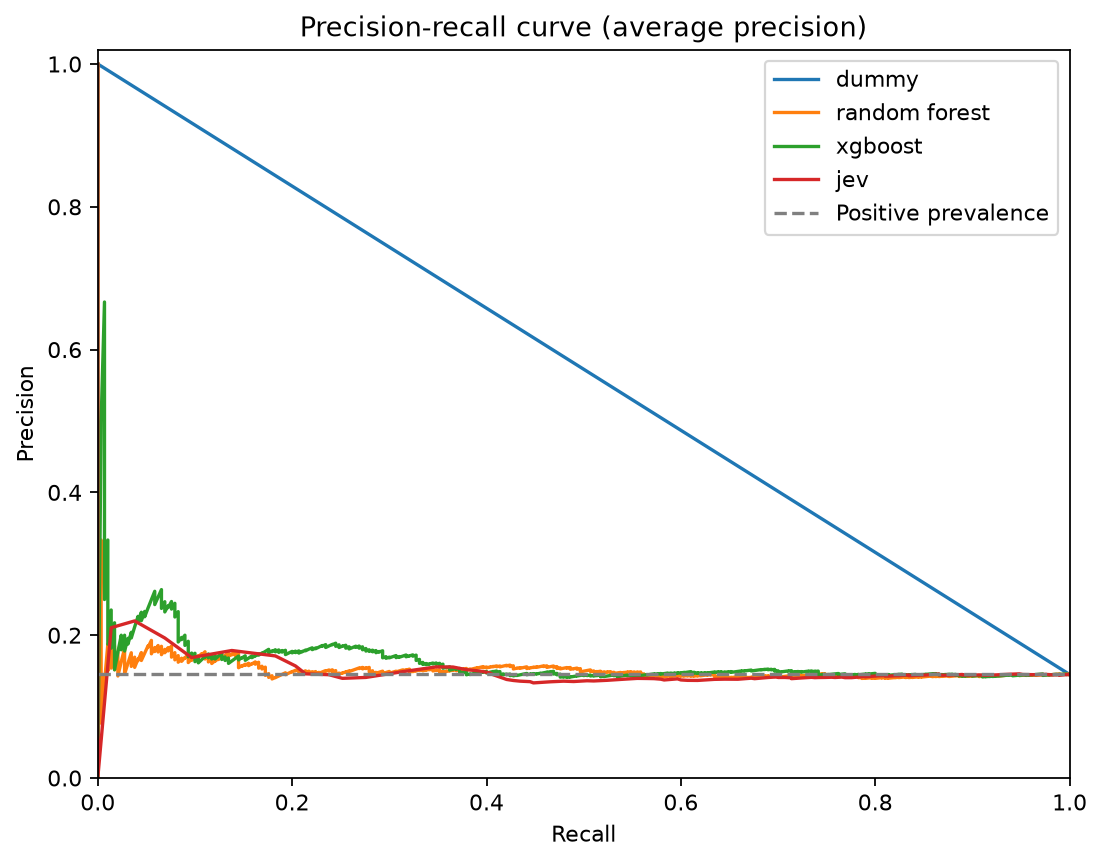
\includegraphics[width=\dimexpr\textwidth-2\fboxsep-2\fboxrule\relax]{original/figures/precision_recall_curve.png}
}\DIFdelendFL \DIFaddbeginFL \DIFaddFL{\includegraphics[width=\dimexpr\textwidth-2\fboxsep-2\fboxrule\relax]{../results/figures/precision_recall_curve.png}
}\DIFaddendFL \caption{Precision--recall curves on the held-out set. The dashed reference is positive prevalence; AP values are reported in Table~\ref{tab:main}. Generated from saved predictions.}\label{fig:pr}
\end{figure}

On probabilistic scoring, Jev's Brier score is 0.459 versus 0.243 for Random Forest, 0.244 for XGBoost, and 0.124 for the constant-prevalence dummy. The paired Jev-minus-XGBoost Brier difference is 0.215 with a 95\% interval of [0.201, 0.230]. The low dummy Brier score makes the central difficulty visible: predicting the base rate is safer under squared error here than these models' poorly informative probability estimates, although the dummy cannot rank or detect individual incidents. Reliability curves (Fig.~\ref{fig:cal}) provide a complementary view; they are descriptive rather than a standalone proof of calibration.

\begin{figure}[t]
\centering
\includegraphics[width=\dimexpr\textwidth-2\fboxsep-2\fboxrule\relax]{../results/figures/calibration_curve.png}
\caption{Positive-class reliability curves with ten quantile bins per model. The diagonal represents perfect calibration. Points have different mean predicted scores across models; empty bins are omitted by the plotting procedure.}\label{fig:cal}
\end{figure}

\DIFaddbegin \subsection{\DIFadd{Probability-Threshold Sensitivity}}\label{sec:thresholds}

\DIFadd{The nine exploratory operating points show how alert volume changes without altering ranking. At $u=0.1$, both trees flag every record (precision 0.145, recall 1.000); at $u=0.9$, both flag none (recall 0 and accuracy 0.855). At $u=0.6$, XGBoost precision rises to 0.333, but only 9 records are flagged and 3 incidents detected (recall 0.010); Random Forest flags one record and detects no incident. Jev's alert rate falls from 0.943 to 0.213 across the endpoint thresholds, while precision is 0.146 at both and recall falls from 0.948 to 0.214. Its thresholded decision at $u=0.5$ has accuracy 0.342, slightly different from its returned-choice accuracy of 0.339. The two decisions agree on 99.75\% of rows; all discrepancies occur at tied probabilities of 0.5. We preserve the primary choice-based result. All nine thresholds are exported in }\path{probability_thresholds.csv}\DIFadd{. These descriptions do not identify an independently validated optimum.
}

\DIFaddend \subsection{Confidence-Based Deferral and Latency}\DIFaddbegin \label{sec:deferral}
\DIFaddend 

Table~\ref{tab:selective} shows that increasing the Jev confidence cutoff reduces \DIFdelbegin \DIFdel{accepted-case }\DIFdelend coverage from 63.7\% at 0.50 to 1.65\% at 0.95. \DIFdelbegin \DIFdel{At every listed cutoff, }\DIFdelend \DIFaddbegin \DIFadd{Every listed }\DIFaddend accepted-case accuracy (\DIFdelbegin \DIFdel{0.272}\DIFdelend \DIFaddbegin \DIFadd{0.273}\DIFaddend --0.310) is below \DIFdelbegin \DIFdel{its unfiltered }\DIFdelend \DIFaddbegin \DIFadd{unfiltered accuracy (}\DIFaddend 0.339\DIFdelbegin \DIFdel{accuracy; thus these thresholds do not yield a monotonic accuracy--coverage improvement. F1 increases at some cutoffs , but class composition changes among accepted records and the number sent for review grows sharply. At 0.90, only 194 }\DIFdelend \DIFaddbegin \DIFadd{). At $t=0.50$, the paired accepted-minus-unfiltered accuracy difference is $-0.037$ (95\% interval }[\DIFadd{$-0.053,-0.021$}]\DIFadd{); at $t=0.80$, it is $-0.059$ }[\DIFadd{$-0.089,-0.029$}]\DIFadd{. The differences at 0.90 and 0.95 have wider intervals spanning zero: }[\DIFadd{$-0.098,0.023$}] \DIFadd{and }[\DIFadd{$-0.213,0.087$}]\DIFadd{. All six cutoffs have 1,000 valid conditional bootstrap draws. At 0.95, only 33 }\DIFaddend cases are retained and 1,\DIFdelbegin \DIFdel{806 }\DIFdelend \DIFaddbegin \DIFadd{967 }\DIFaddend are deferred; \DIFdelbegin \DIFdel{at 0.95, only 33 are retained. These are descriptive comparisons on }\DIFdelend \DIFaddbegin \DIFadd{the accuracy interval }[\DIFadd{0.128, 0.429}] \DIFadd{makes the limited precision of that estimate explicit. F1 increases at some cutoffs, but these changes concern different }\DIFaddend selected subsets, not \DIFdelbegin \DIFdel{estimates of how a }\DIFdelend \DIFaddbegin \DIFadd{a measured improvement in a }\DIFaddend staffed review workflow\DIFdelbegin \DIFdel{would perform}\DIFdelend .

\begin{table}[t]
\caption{Jev selective prediction \DIFaddbeginFL \DIFaddFL{and subset composition}\DIFaddendFL . \DIFaddbeginFL \DIFaddFL{Prev. is accepted-subset incident prevalence; Flag is its predicted-positive fraction. }\DIFaddendFL Accuracy \DIFdelbeginFL \DIFdelFL{, precision, recall, and F1 }\DIFdelendFL \DIFaddbeginFL \DIFaddFL{intervals }\DIFaddendFL are \DIFdelbeginFL \DIFdelFL{conditional on accepted cases; review }\DIFdelendFL \DIFaddbeginFL \DIFaddFL{pointwise percentile bootstrap 95\% intervals. Review }\DIFaddendFL count \DIFdelbeginFL \DIFdelFL{includes all rejected cases}\DIFdelendFL \DIFaddbeginFL \DIFaddFL{is $2{,}000-N$}\DIFaddendFL . \DIFdelbeginFL \DIFdelFL{The unfiltered Jev }\DIFdelendFL \DIFaddbeginFL \DIFaddFL{Unfiltered }\DIFaddendFL accuracy/F1 are .339/.235.}\label{tab:selective}
\centering\DIFdelbeginFL %DIFDELCMD < \scriptsize
%DIFDELCMD < %%%
\DIFdelendFL \DIFaddbeginFL \small
\DIFaddendFL \resizebox{\textwidth}{!}{\begin{tabular}{rrrrrrr}
\hline
Confidence $t$ & Coverage & \DIFdelbeginFL \DIFdelFL{Accepted }\DIFdelendFL \DIFaddbeginFL \DIFaddFL{$N$ }\DIFaddendFL & \DIFdelbeginFL \DIFdelFL{Review }\DIFdelendFL \DIFaddbeginFL \DIFaddFL{Prev. }\DIFaddendFL & \DIFdelbeginFL \DIFdelFL{Accuracy }\DIFdelendFL \DIFaddbeginFL \DIFaddFL{Flag }& \DIFaddFL{Accuracy }[\DIFaddFL{95\% CI}] \DIFaddendFL & \DIFdelbeginFL \DIFdelFL{Precision }%DIFDELCMD < & %%%
\DIFdelFL{Recall / }\DIFdelendFL F1 \\
\hline
.50 & .637 & 1,274 & \DIFdelbeginFL \DIFdelFL{726 }\DIFdelendFL \DIFaddbeginFL \DIFaddFL{.139 }\DIFaddendFL & \DIFaddbeginFL \DIFaddFL{.763 }& \DIFaddendFL .302 \DIFaddbeginFL [\DIFaddFL{.275, .329}] \DIFaddendFL & \DIFdelbeginFL \DIFdelFL{.134 }%DIFDELCMD < & %%%
\DIFdelFL{.734 / }\DIFdelendFL .226 \\
.60 & .548 & 1,096 & \DIFdelbeginFL \DIFdelFL{904 }\DIFdelendFL \DIFaddbeginFL \DIFaddFL{.144 }\DIFaddendFL & \DIFaddbeginFL \DIFaddFL{.765 }& \DIFaddendFL .308 \DIFaddbeginFL [\DIFaddFL{.279, .338}] \DIFaddendFL & \DIFdelbeginFL \DIFdelFL{.142 }%DIFDELCMD < & %%%
\DIFdelFL{.753 / }\DIFdelendFL .239 \\
.70 & .435 & 869 & \DIFdelbeginFL \DIFdelFL{1,131 }\DIFdelendFL \DIFaddbeginFL \DIFaddFL{.157 }\DIFaddendFL & \DIFaddbeginFL \DIFaddFL{.778 }& \DIFaddendFL .310 \DIFaddbeginFL [\DIFaddFL{.278, .342}] \DIFaddendFL & \DIFdelbeginFL \DIFdelFL{.157 }%DIFDELCMD < & %%%
\DIFdelFL{.779 / }\DIFdelendFL .261 \\
.80 & .286 & 571 & \DIFdelbeginFL \DIFdelFL{1,429 }\DIFdelendFL \DIFaddbeginFL \DIFaddFL{.140 }\DIFaddendFL & \DIFaddbeginFL \DIFaddFL{.807 }& \DIFaddendFL .280 \DIFaddbeginFL [\DIFaddFL{.244, .318}] \DIFaddendFL & \DIFdelbeginFL \DIFdelFL{.141 }%DIFDELCMD < & %%%
\DIFdelFL{.813 / }\DIFdelendFL .240 \\
.90 & .097 & 194 & \DIFdelbeginFL \DIFdelFL{1,806 }\DIFdelendFL \DIFaddbeginFL \DIFaddFL{.175 }\DIFaddendFL & \DIFaddbeginFL \DIFaddFL{.814 }& \DIFaddendFL .299 \DIFaddbeginFL [\DIFaddFL{.238, .361}] \DIFaddendFL & \DIFdelbeginFL \DIFdelFL{.177 }%DIFDELCMD < & %%%
\DIFdelFL{.824 / }\DIFdelendFL .292 \\
.95 & .017 & 33 & \DIFdelbeginFL \DIFdelFL{1,967 }\DIFdelendFL \DIFaddbeginFL \DIFaddFL{.242 }\DIFaddendFL & \DIFaddbeginFL \DIFaddFL{.788 }& \DIFaddendFL .273 \DIFaddbeginFL [\DIFaddFL{.128, .429}] \DIFaddendFL & \DIFdelbeginFL \DIFdelFL{.192 }%DIFDELCMD < & %%%
\DIFdelFL{.625 / }\DIFdelendFL .294 \\
\hline
\end{tabular}}
\end{table}

\DIFaddbegin \DIFadd{Confidence--correctness AUC is 0.434 }[\DIFadd{0.407, 0.461}]\DIFadd{, indicating that higher confidence ranks correct decisions below incorrect ones more often than the reverse on these records. Mean confidence is 0.530 for correct decisions and 0.598 for incorrect ones. At $t=0.80$, the accepted subset is 80.7\% predicted positive but only 14.0\% actually positive, with 396 false positives among 571 accepted records. This imbalance explains the observed accepted-case error composition; it does not identify the model's internal cause of failure. Expected accuracy under random acceptance is 0.339 at every nonzero coverage. Fig.~\ref{fig:riskcoverage} contrasts that reference with the full confidence-selection curve and pointwise uncertainty at the six cutoffs.
}

\begin{figure}[t]
\centering
\DIFaddFL{\includegraphics[width=.85\textwidth]{../results/figures/risk_coverage.png}
}\caption{\DIFaddFL{Jev accepted-case error versus coverage (lower is better). Tied confidence scores are retained together. The gray band is a pointwise central 95\% random-acceptance reference conditional on the observed test set, not a confidence band. Blue vertical intervals are pointwise bootstrap 95\% intervals at the six fixed cutoffs.}}\label{fig:riskcoverage}
\end{figure}

\DIFadd{All saved confidence scores are within 0.015 of the documented binary formula $|2p-1|$ (mean absolute discrepancy 0.0051). Thus the field largely reflects probability concentration, not an independently measured correctness signal. This is consistent with the interpretation in the prior Jev audit~\mbox{%DIFAUXCMD
\cite{provatas2026systemone}}\hskip0pt%DIFAUXCMD
, but contrasts with that audit's useful error ranking on other tasks. Formula agreement does not validate the probabilities or imply that reversing the score would produce a deployable policy.
}

\DIFaddend For per-record inference, the Random Forest median is 14.8\,ms (p95 14.9\,ms) and the XGBoost median is 1.5\,ms (p95 1.7\,ms). Jev's hosted round-trip median is 264.0\,ms (p95 311.6\,ms). The respective means are 14.6, 1.5, and 270.9\,ms. These values reflect this run and execution environment; the Jev measurement additionally includes service and network time and should not be interpreted as a pure model-compute benchmark.

\section{Discussion}

\subsection{Interpreting the Research Questions}

\textbf{RQ1: classification.} Near-chance ROC-AUC and AP close to prevalence suggest weak ranking signal in the permitted features for this particular split. Jev's high recall follows from flagging most transactions, not from convincing discrimination. The large majority-class accuracy of the dummy shows why an accuracy-only model ranking would misrepresent incident-detection utility. Previous fraud studies using other data and protocols report stronger discrimination~\cite{han2026fusion,fazel2026ebm}; their scores are not directly comparable with a leakage-controlled evaluation of these simulated labels.

\textbf{RQ2: probability reliability.} The Brier scores and reliability plot show that the probabilities from these runs should not be read as dependable individual risk likelihoods. \DIFdelbegin \DIFdel{In particular, a }\DIFdelend \DIFaddbegin \DIFadd{A }\DIFaddend constant prevalence predictor beats every evaluated model on Brier score despite detecting no incidents. \DIFaddbegin \DIFadd{Both trees use imbalance weighting without post-hoc recalibration, so their probability scores are not those of unweighted or recalibrated baselines. }\DIFaddend Calibration and sharpness must be interpreted together; \DIFdelbegin \DIFdel{post-hoc recalibration on an independent calibration set }\DIFdelend \DIFaddbegin \DIFadd{recalibration on independent data }\DIFaddend is a different experiment and cannot create information absent from the \DIFdelbegin \DIFdel{input }\DIFdelend features~\cite{chidambaram2025reassessing,haotian2023recal}.

\textbf{RQ3: selective decisions.} High reported Jev confidence did not identify a subset with higher \DIFdelbegin \DIFdel{accuracy under the evaluated cutoffs. Although some }\DIFdelend \DIFaddbegin \DIFadd{observed accuracy at the six cutoffs. The correctness AUC and subset counts support a more specific diagnosis than coverage loss alone: concentration in the returned distribution is not aligned with correctness, and high-confidence subsets contain many false-positive alerts. Unknown label-generation rules, underspecified observable incident criteria, and domain mismatch are possible explanations, not experimentally separated causes. Some }\DIFaddend accepted-subset F1 values rise, \DIFdelbegin \DIFdel{they are conditional on }\DIFdelend \DIFaddbegin \DIFadd{but they concern }\DIFaddend a changing subset and require deferring most cases\DIFdelbegin \DIFdel{at high thresholds. Independent work on abstention emphasizes the need to quantify costs and review capacityrather than treating rejection as a free gain}\DIFdelend \DIFaddbegin \DIFadd{. Abstention must account for review costs and capacity}\DIFaddend ~\cite{singh2026abstention}. \DIFdelbegin \DIFdel{A recent evaluation of another commercial System-1 model found confidence utility to be task dependent and sensitive to presentation choices}\DIFdelend \DIFaddbegin \DIFadd{The prior Jev audit found useful confidence-based selection on other tasks}\DIFaddend ~\cite{provatas2026systemone}; \DIFdelbegin \DIFdel{this motivates further testing but supplies no validationfor the current Jev confidence field}\DIFdelend \DIFaddbegin \DIFadd{our contrasting result shows why that finding cannot be transferred without task-specific validation}\DIFaddend .

\textbf{RQ4: operation.} Jev's observed round trip is much slower than the local XGBoost measurement\DIFdelbegin \DIFdel{, while Random Forest 's per-row preprocessing/prediction is slower than XGBoost 's in this implementation}\DIFdelend \DIFaddbegin \DIFadd{. Random Forest also takes longer per row than XGBoost here}\DIFaddend . Different timing boundaries, hardware, API load, network path, and batch sizes limit the generality of these numbers. No cost estimate or production-service guarantee follows from this run.

\subsection{Validity and Scope}

First, the publisher describes the dataset as a simulation, but does not publish a verified real-world outcome mechanism. The perfect target encoding in three incident fields demonstrates why feature availability must be specified. It does \emph{not} establish that the remaining 12 fields carry a usable pre-event signal, nor prove that labels were generated independently of them. Thus we cannot attribute the weak discrimination to any one model architecture. Second, one random stratified split of one dataset does not estimate temporal generalization, robustness to changed prevalence, or variability over data splits. Bootstrap intervals quantify uncertainty conditional on this frozen test set and fixed predictions.

Third, the methods receive unequal supervision: the trees see 8,000 labeled records, while Jev sees one record at a time with no examples. No Jev model card or training-data audit was available to establish what the hosted system may have encountered during pretraining. Its alias can change; the returned version and prompt version are recorded for this run. The question asks whether a row \emph{should} be flagged without an externally validated rule linking its observable fields to the synthetic incident label. More detailed incident criteria cannot be reconstructed from the excluded post-event fields without leakage. Fourth, \DIFdelbegin \DIFdel{the Jev}\DIFdelend \DIFaddbegin \DIFadd{Jev's }\DIFaddend hard choice need not coincide with thresholding its \DIFdelbegin \DIFdel{reported }\DIFdelend positive-class probability at 0.5; we \DIFdelbegin \DIFdel{respect the returned decision rather than retrofitting a test-set threshold. Selected-case metrics at the six cutoffs have no separate selection datasetand should not be presented as a deployable deferral policy}\DIFdelend \DIFaddbegin \DIFadd{preserve that distinction. The revision's probability-threshold and confidence diagnostics reuse the existing test predictions, with no independent selection dataset. Their intervals are pointwise and exploratory; in particular, apparent gains from intermediate thresholds, reversing confidence, or inspecting many cutoffs would need independent validation}\DIFaddend . Human reviewers, error costs, and downstream actions were not measured.

Finally, the tabular foundation model and LLM studies cited above involve different architectures, context regimes, and datasets~\cite{hollmann2025tabpfn,grushina2026llmtab,garnelo2026tabular}. Their mixed evidence motivates careful evaluation, not a transfer of their performance claims to Jev. Likewise, protocol-sensitive risk benchmarking elsewhere~\cite{mishra2026erp,zeng2026fraudbench} reinforces the need to keep leakage control and dataset provenance explicit when interpreting this negative finding.

\section{Conclusion}

On a shared, leakage-aware evaluation of simulated accounting transactions, Jev, Random Forest, and XGBoost all yield ROC-AUC values near chance after target-encoding fields are removed. Jev flags many more cases and attains higher recall, but at low precision and a substantially worse Brier score than the local models\DIFdelbegin \DIFdel{; its reported confidence does not improve accepted-case accuracy at the tested cutoffs }\DIFdelend \DIFaddbegin \DIFadd{. Offline threshold analysis exposes alert-volume trade-offs, while confidence-error ranking and accepted-subset composition explain why the six evaluated deferral cutoffs do not increase observed accuracy}\DIFaddend . These observations bound \DIFdelbegin \DIFdel{what can be claimed from the experiment: neither the hosted decision service nor the supervised baselines demonstrate }\DIFdelend \DIFaddbegin \DIFadd{the contribution: none of the evaluated settings demonstrates }\DIFaddend reliable individual incident screening on the permitted features \DIFdelbegin \DIFdel{. A useful next study would test independently justified pre-event risk criteria and additional }\DIFdelend \DIFaddbegin \DIFadd{of this dataset.
}

\textbf{\DIFadd{Future work.}} \DIFadd{Evaluation should extend to multiple real-world accounting and fraud }\DIFaddend datasets with documented label \DIFdelbegin \DIFdel{generation, while fixing prompts, thresholds, }\DIFdelend \DIFaddbegin \DIFadd{provenance and verified pre-event feature availability, using temporal and entity-separated splits where appropriate. Simulation studies should publish their generator and vary signal strength, imbalance, and incident mechanisms rather than treating one synthetic file as representative. Further experiments should define observable risk criteria independently, compare supervision-matched settings, and use separate validation/calibration data to fix prompts, probability thresholds, confidence policies, }\DIFaddend and review budgets before \DIFdelbegin \DIFdel{examining test labels. }\DIFdelend \DIFaddbegin \DIFadd{testing. Repeated splits and service calls would quantify additional variability; cost-sensitive evaluation with actual reviewers would be required to assess an operational deferral workflow.
}\DIFaddend 

\DIFaddbegin \section*{\DIFadd{Acknowledgements}}

\textbf{\DIFadd{Funding and conflicts of interest.}} \DIFadd{This research received no external funding. The authors declare no conflicts of interest.
}

\textbf{\DIFadd{Contributorship.}} \DIFadd{Yehezkiel Gunawan: conceptualization, formal analysis, investigation, methodology, resources, visualization, writing, and editing. Tanty Oktavia: conceptualization, formal analysis, project administration, validation, and review.
}

\textbf{\DIFadd{Open data.}} \DIFadd{The authors acknowledge Ziya for making the Financial Transaction and Risk Management Dataset openly available on Kaggle under the CC0 Public Domain license~\mbox{%DIFAUXCMD
\cite{ziya2025dataset}}\hskip0pt%DIFAUXCMD
. The dataset used in this study is available from its original source at }\url{https://www.kaggle.com/datasets/ziya07/financial-transaction-and-risk-management-dataset}\DIFadd{.
}

\DIFaddend \section*{AI Usage Declaration}
Generative AI tools were used to assist with coding the experimental pipeline and to paraphrase and improve the language of the manuscript. They also assisted with organizing evidence and preparing an initial manuscript draft and bibliography. The authors reviewed the experimental code and are responsible for verifying the data, results, references, figures, interpretations, and final wording. Generative AI did not generate the research data or experimental figures.


\begin{thebibliography}{10}
\providecommand{\url}[1]{\texttt{#1}}
\providecommand{\urlprefix}{URL }
\providecommand{\doi}[1]{https://doi.org/#1}

\bibitem{breiman2001forests}
Breiman, L.: Random forests. Machine Learning  \textbf{45}(1),  5--32 (2001).
  \doi{10.1023/A:1010933404324}

\bibitem{chen2016xgboost}
Chen, T., Guestrin, C.: {XGBoost}: A scalable tree boosting system. In:
  Proceedings of the 22nd ACM SIGKDD International Conference on Knowledge
  Discovery and Data Mining. pp. 785--794 (2016). \doi{10.1145/2939672.2939785}

\bibitem{chidambaram2025reassessing}
Chidambaram, M., Ge, R.: Reassessing how to compare and improve the calibration
  of machine learning models. In: International Conference on Learning
  Representations (2025), \url{https://arxiv.org/abs/2406.04068}

\DIFaddbegin \bibitem{dalpozzolo2018fraud}
\DIFadd{Dal~Pozzolo, A., Boracchi, G., Caelen, O., Alippi, C., Bontempi, G.: Credit
  card fraud detection: A realistic modeling and a novel learning strategy.
  IEEE Transactions on Neural Networks and Learning Systems  }\textbf{29}(8)\DIFadd{,
  3784--3797 (2018). }\doi{10.1109/TNNLS.2017.2736643}

\DIFaddend \bibitem{davis2006pr}
Davis, J., Goadrich, M.H.: The relationship between precision-recall and {ROC}
  curves. In: Proceedings of the 23rd International Conference on Machine
  Learning. pp. 233--240 (2006). \doi{10.1145/1143844.1143874}

\bibitem{fazel2026ebm}
Fazel, R.E., Bakhtiary, A., Bigdeli, S.A.: Improving credit card fraud
  detection with an optimized explainable boosting machine. arXiv preprint
  arXiv:2602.06955 (2026), \url{https://arxiv.org/abs/2602.06955}

\bibitem{garnelo2026tabular}
Garnelo, M., Czarnecki, W.M.: Why large language models fail at tabular
  prediction. arXiv preprint arXiv:2608.02412 (2026),
  \url{https://arxiv.org/abs/2608.02412}

\DIFaddbegin \bibitem{geifman2017selective}
\DIFadd{Geifman, Y., El-Yaniv, R.: Selective classification for deep neural networks.
  In: Advances in Neural Information Processing Systems. vol.~30 (2017),
  }\url{https://proceedings.neurips.cc/paper/2017/hash/4a8423d5e91fda00bb7e46540e2b0cf1-Abstract.html}

\DIFaddend \bibitem{grinsztajn2022trees}
Grinsztajn, L., Oyallon, E., Varoquaux, G.: Why do tree-based models still
  outperform deep learning on tabular data? In: Advances in Neural Information
  Processing Systems. vol.~35 (2022), \url{https://arxiv.org/abs/2207.08815}

\bibitem{grushina2026llmtab}
Grushina, D., Kuvshinova, K., Kostromina, A., Temirkhanov, A., Mitrovic, M.,
  Simakov, D.: \DIFaddbegin \DIFadd{Do you even need more data? rethinking }\DIFaddend {LLM\DIFdelbegin \DIFdel{TabBench}\DIFdelend  } \DIFdelbegin \DIFdel{: Evaluating }\DIFdelend \DIFaddbegin \DIFadd{deployment for
  label-scarce tabular classification with }\DIFaddend {\DIFdelbegin \DIFdel{LLMs}\DIFdelend \DIFaddbegin \DIFadd{TabLens}\DIFaddend }\DIFdelbegin \DIFdel{on binary tabular classification from zero to few shots}\DIFdelend . arXiv preprint
  arXiv:2605.24417\DIFaddbegin \DIFadd{, version 3 }\DIFaddend (2026), \DIFdelbegin %DIFDELCMD < \url{https://arxiv.org/abs/2605.24417}
%DIFDELCMD < %%%
\DIFdelend \DIFaddbegin \url{https://arxiv.org/abs/2605.24417v3}
\DIFaddend 

\bibitem{guo2017calibration}
Guo, C., Pleiss, G., Sun, Y., Weinberger, K.Q.: On calibration of modern neural
  networks. In: Proceedings of the 34th International Conference on Machine
  Learning. Proceedings of Machine Learning Research, vol.~70, pp. 1321--1330
  (2017), \url{https://proceedings.mlr.press/v70/guo17a.html}

\bibitem{han2026fusion}
Han, X., Wu, C.: Validation-stage combinatorial fusion analysis for imbalanced
  credit-card fraud detection. arXiv preprint arXiv:2606.10393 (2026),
  \url{https://arxiv.org/abs/2606.10393}

\bibitem{haotian2023recal}
HaoTian, W., Zhang, Z., Hu, M., Wang, Q., Chen, L., Bian, Y., Wu, B.: {RECAL}:
  Sample-relation guided confidence calibration over tabular data. In: Findings
  of the Association for Computational Linguistics: EMNLP 2023. pp. 7246--7257
  (2023). \doi{10.18653/v1/2023.findings-emnlp.482}

\bibitem{hollmann2025tabpfn}
Hollmann, N., M{\"u}ller, S., Purucker, L., Krishnakumar, A., K{\"o}rfer, M.,
  Hoo, S.B., Schirrmeister, R.T., Hutter, F.: Accurate predictions on small
  data with a tabular foundation model. Nature  \textbf{637},  319--326 (2025).
  \doi{10.1038/s41586-024-08328-6}

\DIFaddbegin \bibitem{kaufman2012leakage}
\DIFadd{Kaufman, S., Rosset, S., Perlich, C., Stitelman, O.: Leakage in data mining:
  Formulation, detection, and avoidance. ACM Transactions on Knowledge
  Discovery from Data  }\textbf{6}(4)\DIFadd{,  1--21 (2012).
  }\doi{10.1145/2382577.2382579}

\DIFaddend \bibitem{mcelfresh2023tabzilla}
McElfresh, D., Khandagale, S., Valverde, J., Prasad~C, V., Feuer, B., Hegde,
  C., Ramakrishnan, G., Goldblum, M., White, C.: When do neural nets outperform
  boosted trees on tabular data? In: Advances in Neural Information Processing
  Systems: Datasets and Benchmarks Track (2023),
  \url{https://arxiv.org/abs/2305.02997}

\bibitem{mishra2026erp}
Mishra, S.: {ERP-RiskBench}: Leakage-safe ensemble learning for financial risk.
  arXiv preprint arXiv:2603.06671 (2026),
  \url{https://arxiv.org/abs/2603.06671}

\bibitem{provatas2026systemone}
Provatas, K.A., Georgakopoulos-Soares, I.: Auditing system-1 models on
  biosecurity-relevant benchmarks: Calibration, selective prediction, and
  permutation instability in a non-generative model. arXiv preprint
  arXiv:2609.30454 (2026), \url{https://arxiv.org/abs/2609.30454}

\bibitem{singh2026abstention}
Singh, M., Srikantha, A., Lakhanpal, S.: Cost-sensitive conformal prediction
  and human-in-the-loop abstention for imbalanced high-stakes decision support:
  A multi-domain benchmark. arXiv preprint arXiv:2607.27143 (2026),
  \url{https://arxiv.org/abs/2607.27143}
\DIFaddbegin 

\bibitem{typesafe2026choice}
{\DIFadd{TypeSafe}}\DIFadd{: Choice: System one api documentation (2026),
  }\url{https://docs.typesafe.ai/primitives/choice}\DIFadd{, vendor documentation;
  accessed 1 November 2026
}

\bibitem{typesafe2026confidence}
{\DIFadd{TypeSafe}}\DIFadd{: Confidence: How typesafe reports certainty (2026),
  }\url{https://docs.typesafe.ai/confidence}\DIFadd{, vendor documentation; accessed 1
  November 2026
}\DIFaddend 

\bibitem{zeng2026fraudbench}
Zeng, X., Bi, Z., Yang, Y., Chen, H., Sheng, Q.Z.: {FraudBench}:
  Protocol-sensitive benchmarking of adversarial robustness for financial risk
  assessment. arXiv preprint arXiv:2608.24551 (2026),
  \url{https://arxiv.org/abs/2608.24551}

\bibitem{ziya2025dataset}
{Ziya}: Financial transaction and risk management dataset. Kaggle, version 1,
  CC0 Public Domain (2025),
  \url{https://www.kaggle.com/datasets/ziya07/financial-transaction-and-risk-management-dataset},
  accessed 28 September 2026

\end{thebibliography}


\end{document}
